\documentclass[12pt,a4paper]{beamer}
%\documentclass[12pt,a4paper,handout]{beamer}
\usetheme{Amsterdam}
%\usecolortheme{beaver}
\usepackage[english,french]{babel}
%\usepackage[utf8]{inputenc}  
\usepackage[T1]{fontenc}
\usepackage{fontspec}
\usepackage{amsmath}
\usepackage{amsfonts}
\usepackage{amssymb}
\usepackage{tikz}
\usepackage{listings}
\usepackage{pgfplots}
%\pgfplotsset{compat=1.14}
\pgfplotsset{compat=newest}

\usepackage{color}
\definecolor{mygreen}{rgb}{0,0.6,0}
\definecolor{mygray}{rgb}{0.5,0.5,0.5}
\definecolor{mymauve}{rgb}{0.58,0,0.82}
\definecolor{greenfluo}{rgb}{0,255,0}
\definecolor{blueemph}{RGB}{17,59,94}


%Underline in color
\newcommand{\coloruline}[3]{\emph{\textcolor{#1}{\underline{#2\textcolor{black}{#3}}}}}

\newcommand{\hl}[1]{\textcolor{blueemph}{#1}}

%
\setbeamertemplate{blocks}[rounded]


\lstset{
  language=Java,
  commentstyle=\color{mygreen},    % comment style
  stringstyle=\color{mymauve},     % string literal style
  keywordstyle=\color{blue},       % keyword style
  basicstyle=\footnotesize        % the size of the fonts that are used for the code
}

\title{\textbf{Algorithmique avancée}}
\subtitle{Algorithmes de tris}
\author{Frédéric Guyomarch}
\date{2018/2019 - Semestre 3}
\institute % (optional)
{

  IUT-A \\
  Université de Lille, Sciences et Technologies

}

 
\logo{\includegraphics[width=5em]{figs/iutaustl}}

%Remove Figure prefix on captures
\setbeamertemplate{caption}{\raggedright\insertcaption\par}

%Remove Control bar
\beamertemplatenavigationsymbolsempty





\begin{document}
%TODO bilan, refaire image car fond jaune dégueu sur chiffres, utiliser calques

\begin{frame}
\titlepage
\end{frame}


\begin{frame}{Qu'est-ce qu'un tri?}

\begin{definition}
Trier, c'est ranger des éléments en respectant un ordre particulier.
\end{definition}
\pause
\begin{center}
Le plus souvent, on trie suivant l'ordre numérique ou lexicographique.
\end{center}

\end{frame}


\begin{frame}{Pourquoi trier?}{Quelques exemples}
Le tri est omniprésent en informatique:
\begin{itemize}
\item Pour améliorer la recherche d'éléments 
  \begin{itemize}
  \item dichotomie sur tableaux ordonnés
  \end{itemize}
\item Pour ranger des éléments en fonction de leurs caractéristiques
  \begin{itemize}
  \item boutique en ligne: tri par prix ou note
  \item emails: tri par taille ou priorité
  \end{itemize}
\end{itemize}
\end{frame}

\begin{frame}{Comparaison d'algorithmes}{Quelques critères}

On peut mesurer l'efficacité d'un algorithme en se penchant sur
\begin{itemize}
\item le nombre d'\hl{étapes} nécessaires,
\item le nombre de \hl{comparaisons} réalisées,
\item le nombre d'\hl{échanges} effectués.
\end{itemize}

\pause
Généralement, on regarde le nombre d'étapes nécessaires dans le pire cas pour comparer deux algorithmes.

\end{frame}

\begin{frame}{Comparaison d'algorithmes}{Exemple}
Rappelez-vous, pour un tableau ordonné:
\begin{itemize}
\item La recherche séquentielle requiert $n$ étapes dans le pire cas.
\item La recherche dichotomique requiert  $log_2 n$ étapes dans le pire cas.
\end{itemize}



\end{frame}

%\begin{frame}{Complexité}{Mesure de l'efficacité d'un algorithme}
%\begin{itemize}
%\item Principal critère pour juger de l'efficacité d'un algorithme.
%\item Borne supérieure sur le nombre nécessaires d'étapes pour traiter des données d'entrée de taille $n$.
%\end{itemize}
%
%Dire qu'un algorithme a une complexité en $\mathcal{O}(n)$ revient à dire que dans le pire cas, il lui faudra $n$ étapes pour traiter une entrée de taille $n$.
%
%
%\end{frame}
%
%
%
%\begin{frame}{Complexité}{Représentation graphique}
%\pagestyle{empty}
%\begin{tikzpicture}
%\begin{axis}[
%	minor tick num=1,
%	axis x line=middle,
%	axis y line=	middle,
%	every inner x axis line/.append style=
%		{|->},
%	every inner y axis line/.append style=
%		{|->},
%	ylabel=$n$ {\'e}tapes,xlabel=$n$ {\'e}l{\'e}ments
%]
%\addplot[blue,domain=0:25] {x} node[pos=5] {$\mathcal{O(n)}$};
%
%\addplot[red,domain=0:25] {x^2} node[pos=5] {$\mathcal{O(n^2)}$};
%\addplot[green,domain=0:25] {x*ln(x)/ln(2} node[pos=5] {$\mathcal{O \log n}$};
%\addplot[orange,domain=0:25] {1} node[pos=5] {$\mathcal{O(1}$};
%
%
%
%\end{axis}
%\end{tikzpicture}
%
%\end{frame}
%
%\begin{frame}{Complexité}{En résumé}
%Grossièrement pour les algorithmes de tris
%\begin{itemize}
%\item [$\mathcal{O}(n)$] Bien!
%\end{itemize}
%
%
%\end{frame}


\begin{frame}{Plan}
Revue de quelques algorithmes de tri:%\newline
%Certains lents:
\begin{itemize}
\item Tri à bulles
\item Tri par sélection
\item Tri par insertion
\end{itemize}
%D'autres plus performants:
%\begin{itemize}
%\item Tri rapide
%\end{itemize}
\end{frame}

\begin{frame}{Le tri à bulles}

\begin{figure}
\centering
\includegraphics[scale=0.5]{figs/bubbles}
\end{figure}

\end{frame}


\begin{frame}{Principe}
\begin{itemize}
\item[1]On compare successivement les cases deux à deux.
\item[2]On échange les valeurs si nécessaires de manière à respecter l'ordre
\item[3]On répète les étapes 1 et 2 conjointement jusqu'à obtenir un tableau trié.
\end{itemize}
%On va  comparer les valeurs deux-à-deux jusqu'à obtenir un tableau trié.\newline

\end{frame}



\begin{frame}{En images}

Un premier tour:

\only<1>{
\begin{figure}
\centering
\includegraphics[scale=0.22]{figs/bubble_sort_2}
\end{figure}
}


\only<2>{
\begin{figure}
\centering
\includegraphics[scale=0.22]{figs/bubble_sort_3}
\end{figure}
}


\only<3>{
\begin{figure}
\centering
\includegraphics[scale=0.22]{figs/bubble_sort_4}
\end{figure}
}


\only<4>{
\begin{figure}
\centering
\includegraphics[scale=0.22]{figs/bubble_sort_5}
\end{figure}
}


\only<5>{
\begin{figure}
\centering
\includegraphics[scale=0.22]{figs/bubble_sort_6}
\end{figure}
}


\only<6>{
\begin{figure}
\centering
\includegraphics[scale=0.22]{figs/bubble_sort_7}
\end{figure}
}


\only<7>{
\begin{figure}
\centering
\includegraphics[scale=0.22]{figs/bubble_sort_8}
\end{figure}
}


\only<8>{
\begin{figure}
\centering
\includegraphics[scale=0.22]{figs/bubble_sort_9}
\end{figure}
}


\only<9>{
\begin{figure}
\centering
\includegraphics[scale=0.22]{figs/bubble_sort_10}
\end{figure}
}


\only<10>{
\begin{figure}
\centering
\includegraphics[scale=0.22]{figs/bubble_sort_11}
\end{figure}
}


\only<11>{
\begin{figure}
\centering
\includegraphics[scale=0.22]{figs/bubble_sort_12}
\end{figure}
}


\only<12>{
\begin{figure}
\centering
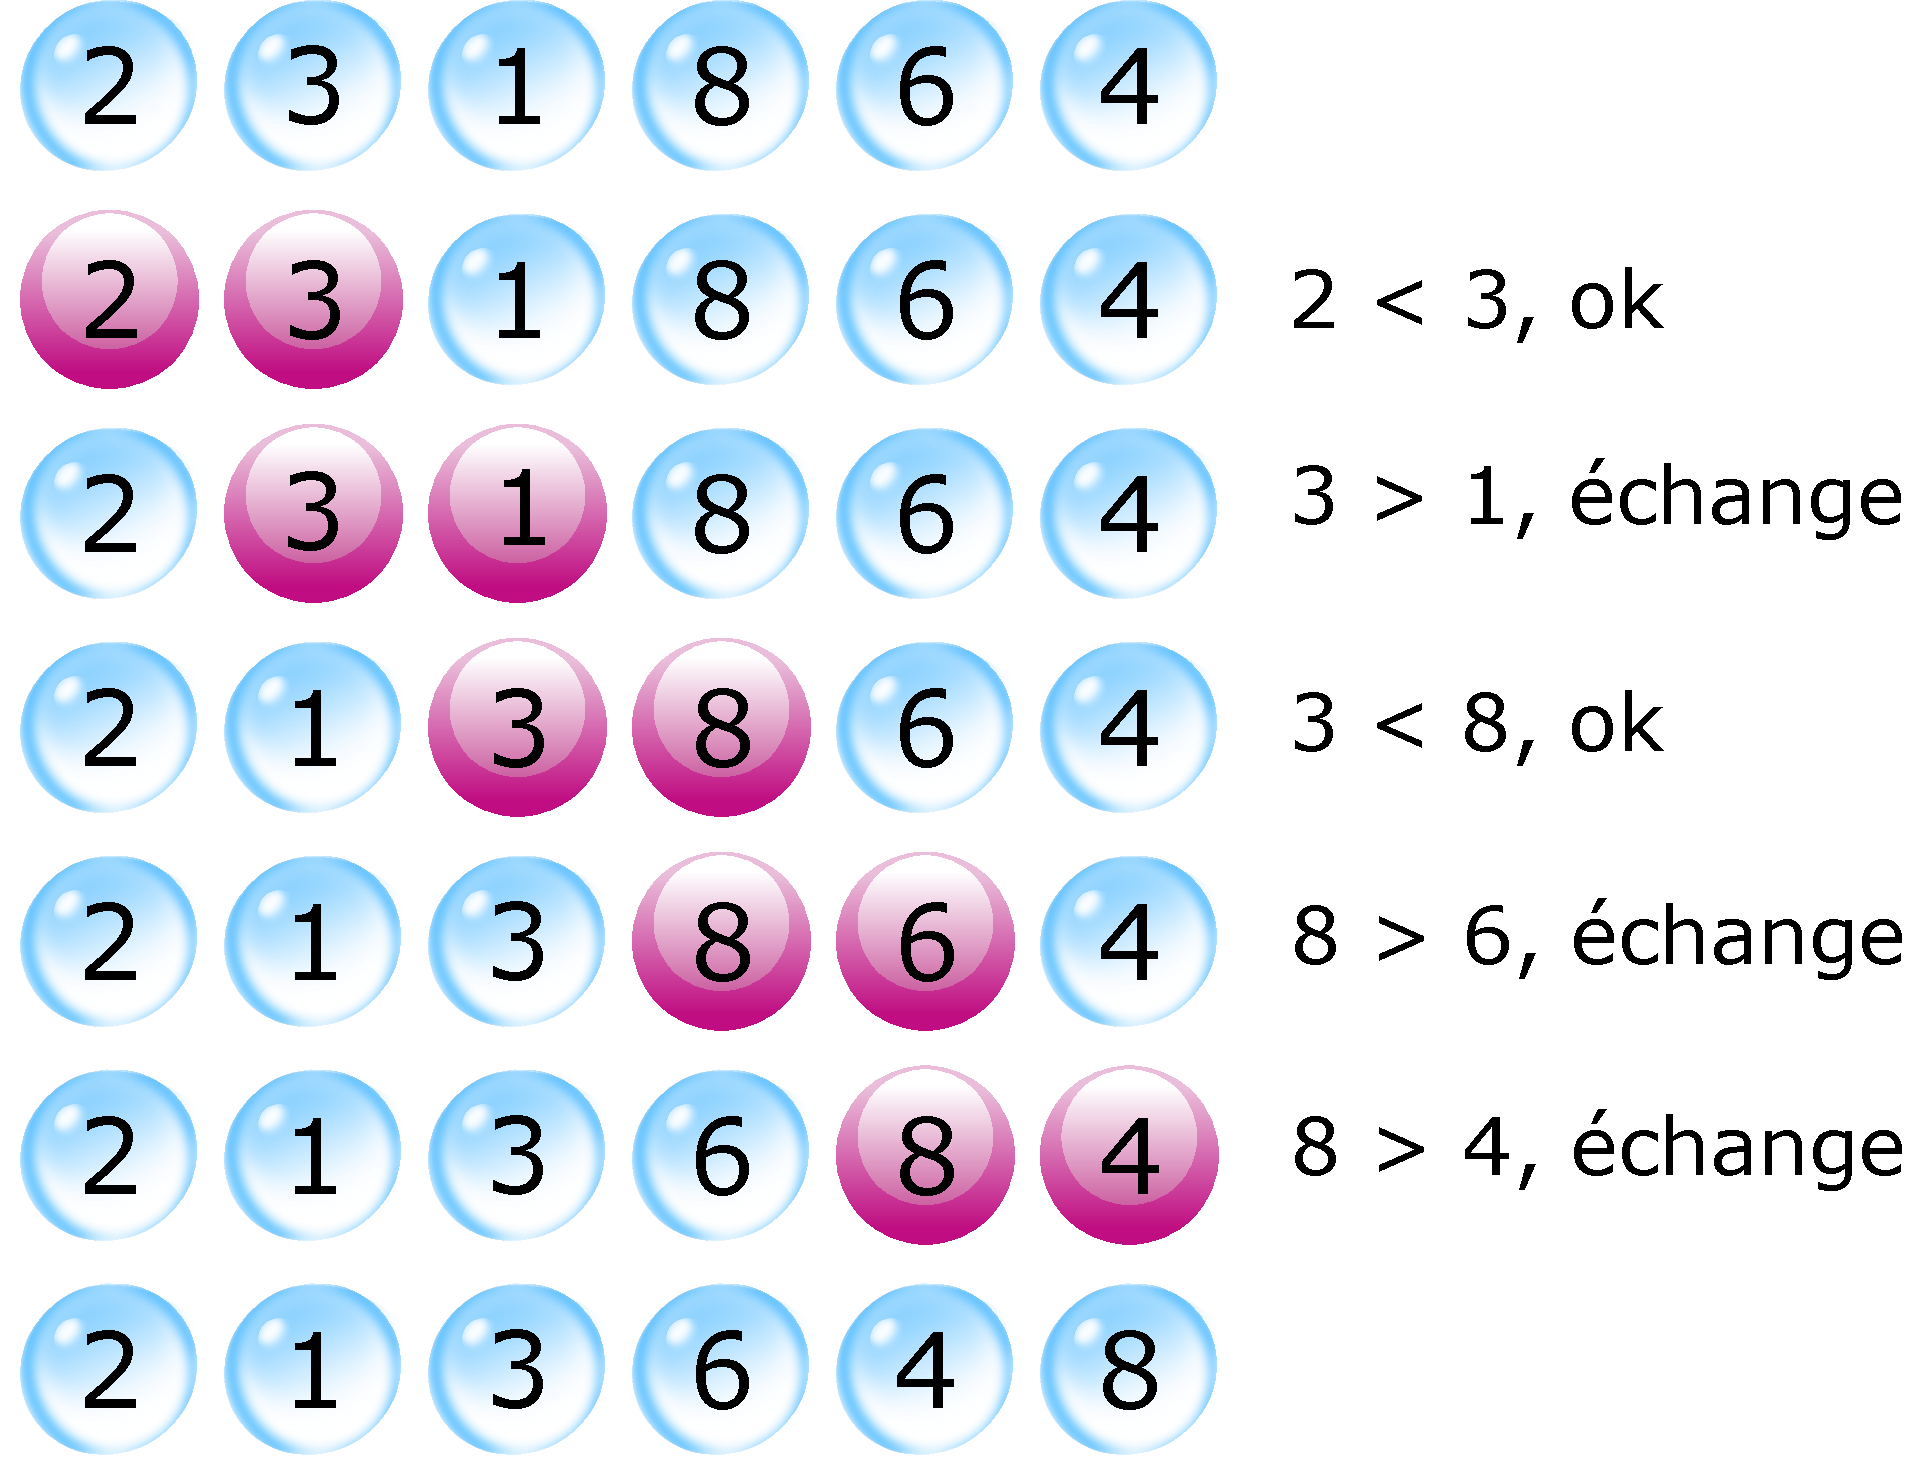
\includegraphics[scale=0.22]{figs/bubble_sort_13}
\end{figure}
}


\only<13>{
\begin{figure}
\centering
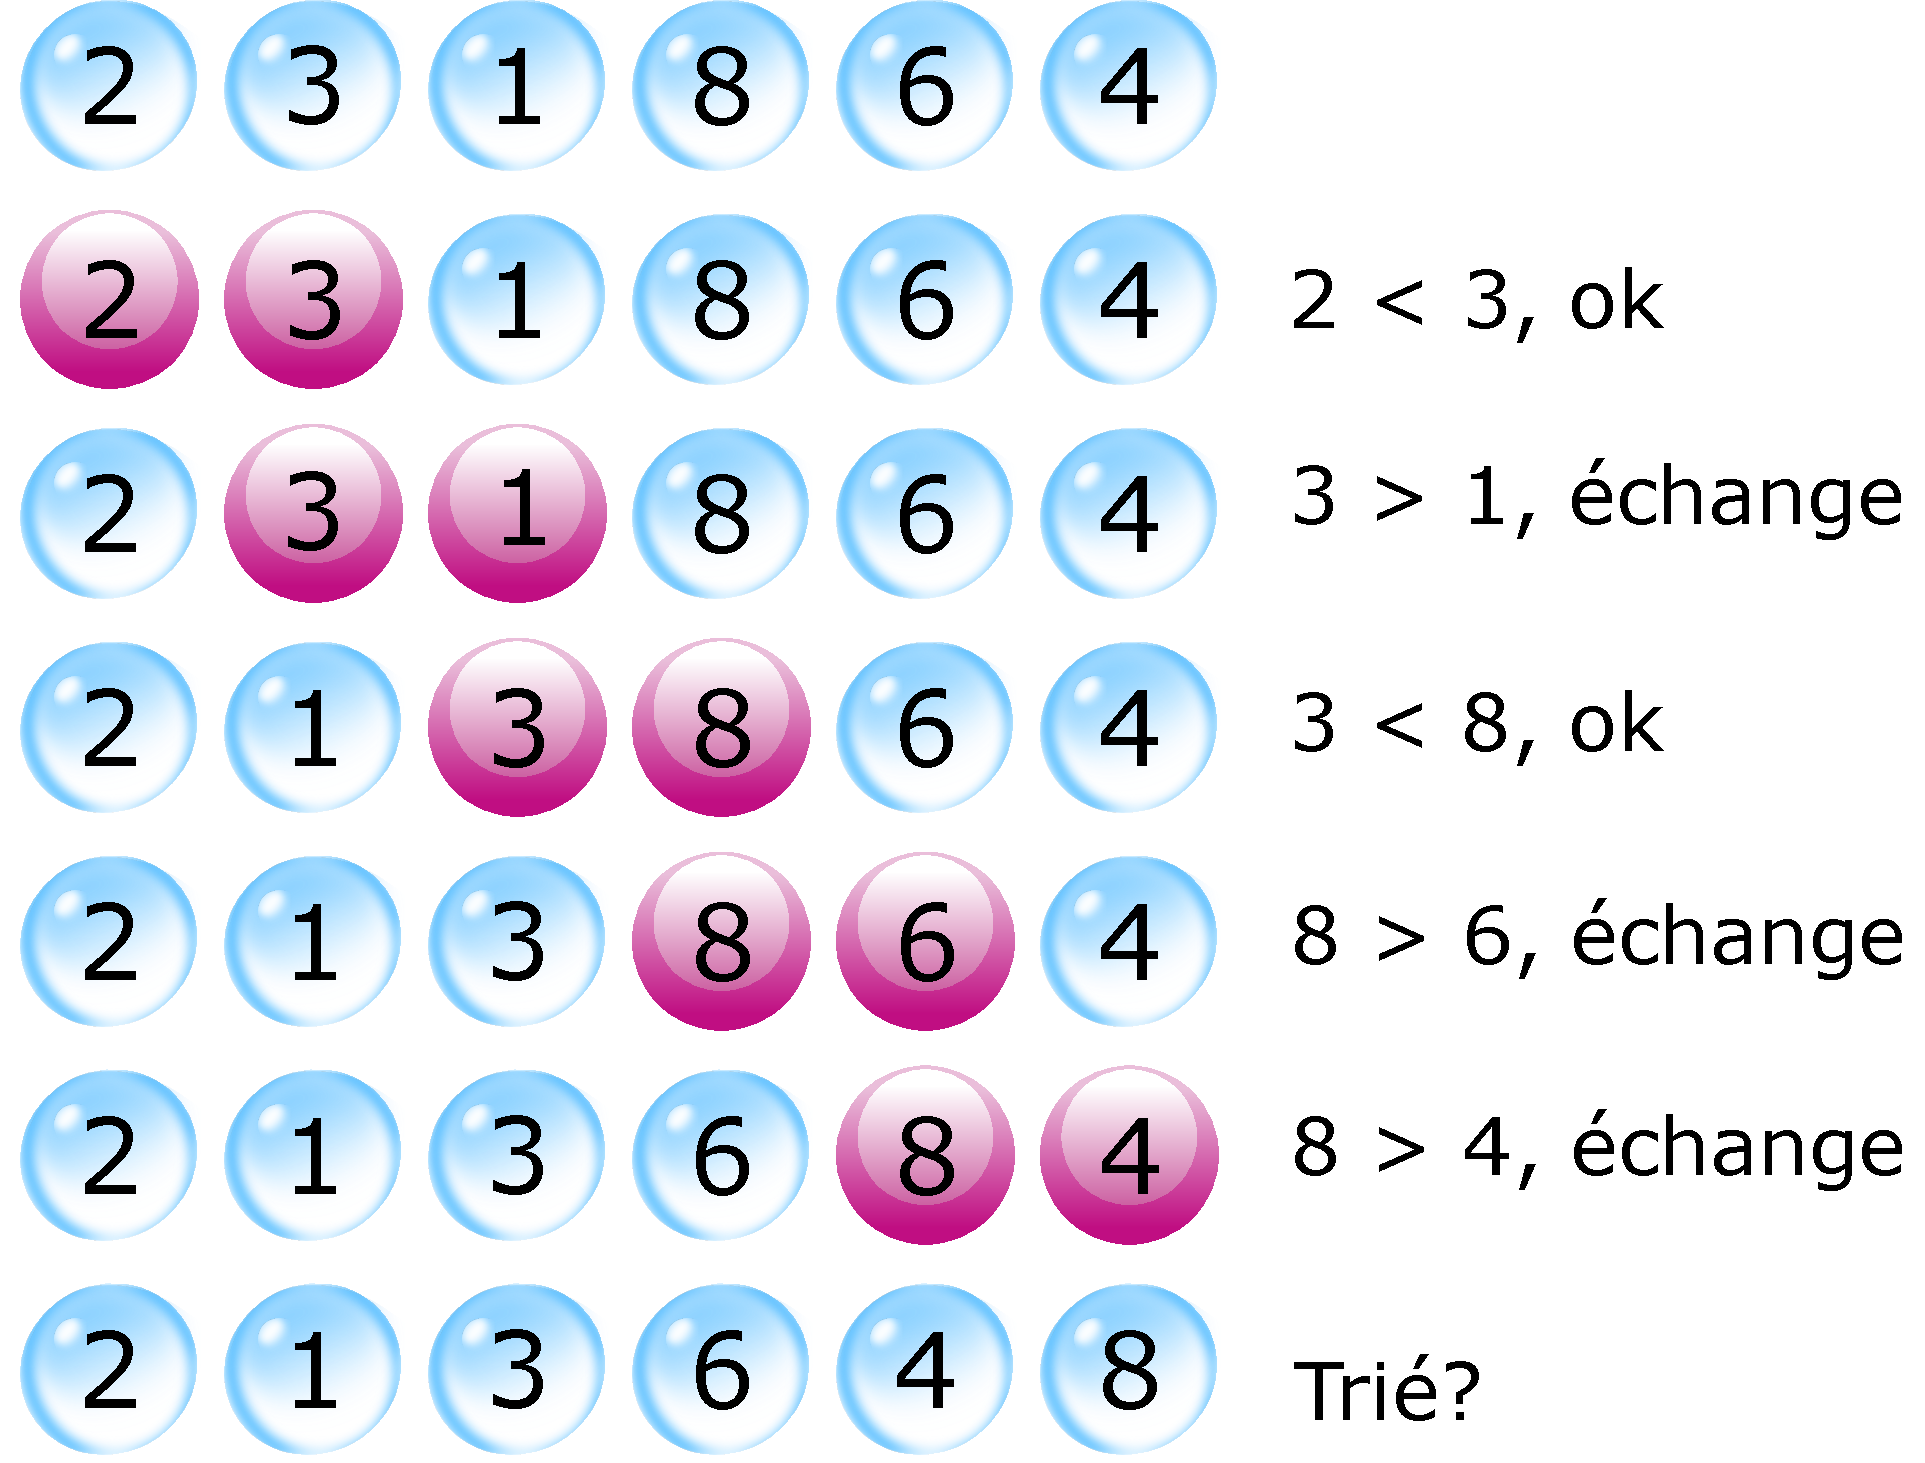
\includegraphics[scale=0.22]{figs/bubble_sort_14}
\end{figure}
}

\end{frame}
\begin{frame}{Principe}
Un deuxième tour:


\only<1>{
\begin{figure}
\centering
\includegraphics[scale=0.22]{figs/bubble_sort2_1}
\end{figure}
}

\only<2>{
\begin{figure}
\centering
\includegraphics[scale=0.22]{figs/bubble_sort2_2}
\end{figure}
}

\only<3>{
\begin{figure}
\centering
\includegraphics[scale=0.22]{figs/bubble_sort2_3}
\end{figure}
}

\only<4>{
\begin{figure}
\centering
\includegraphics[scale=0.22]{figs/bubble_sort2_4}
\end{figure}
}

\only<5>{
\begin{figure}
\centering
\includegraphics[scale=0.22]{figs/bubble_sort2_5}
\end{figure}
}

\only<6>{
\begin{figure}
\centering
\includegraphics[scale=0.22]{figs/bubble_sort2_6}
\end{figure}
}

\only<7>{
\begin{figure}
\centering
\includegraphics[scale=0.22]{figs/bubble_sort2_7}
\end{figure}
}

\only<8>{
\begin{figure}
\centering
\includegraphics[scale=0.22]{figs/bubble_sort2_8}
\end{figure}
}

\only<9>{
\begin{figure}
\centering
\includegraphics[scale=0.22]{figs/bubble_sort2_9}
\end{figure}
}

\only<10>{
\begin{figure}
\centering
\includegraphics[scale=0.22]{figs/bubble_sort2_10}
\end{figure}
}

\only<11>{
\begin{figure}
\centering
\includegraphics[scale=0.22]{figs/bubble_sort2_11}
\end{figure}
}

\only<12>{
\begin{figure}
\centering
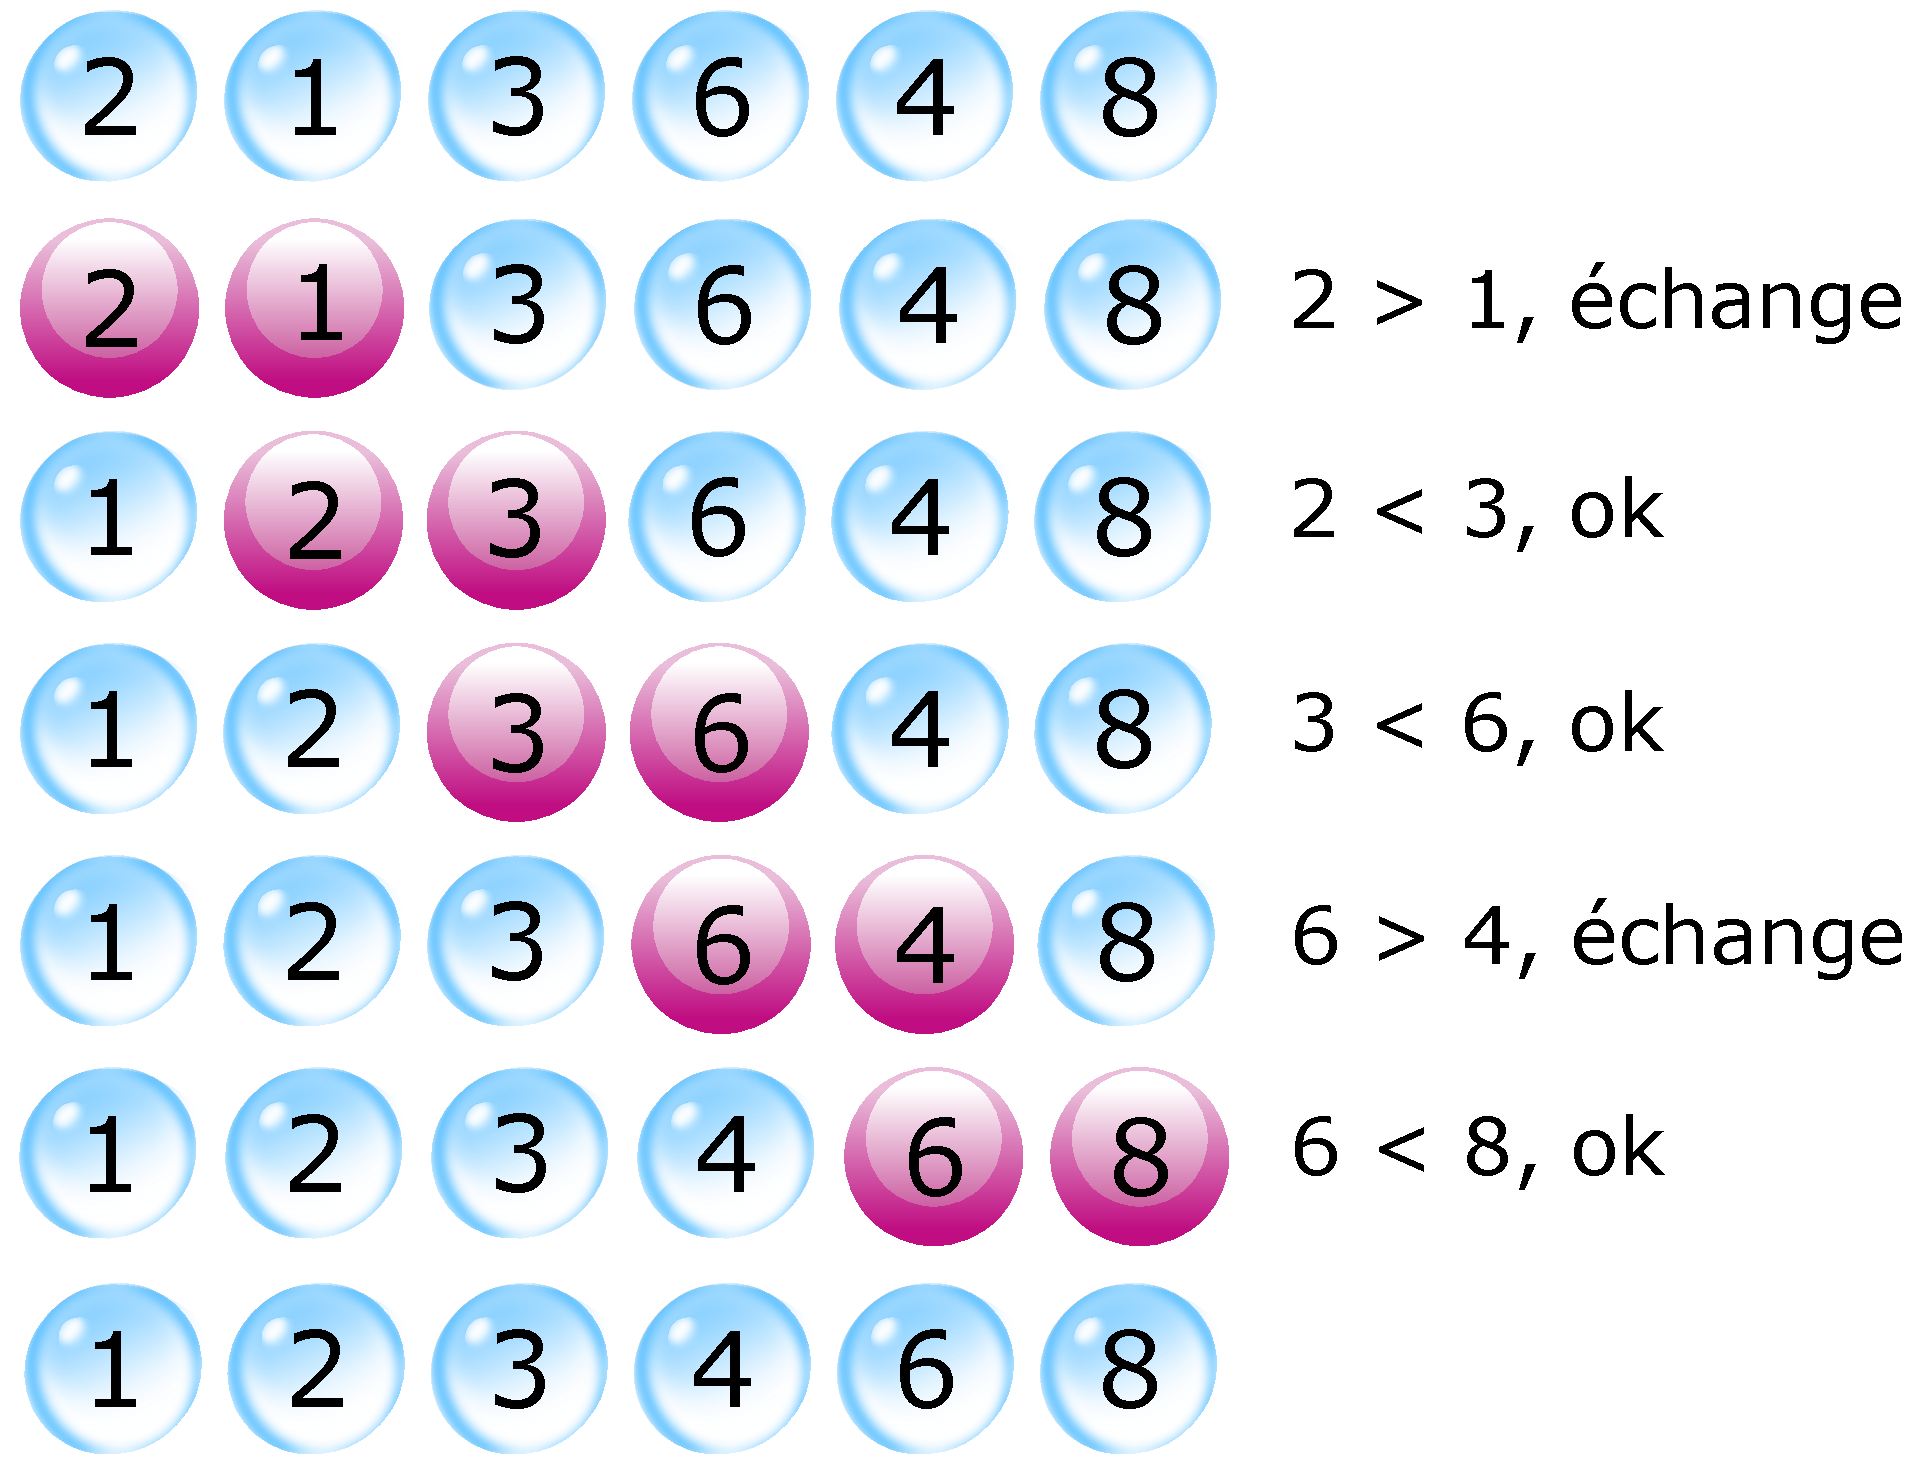
\includegraphics[scale=0.22]{figs/bubble_sort2_12}
\end{figure}
}

\only<13>{
\begin{figure}
\centering
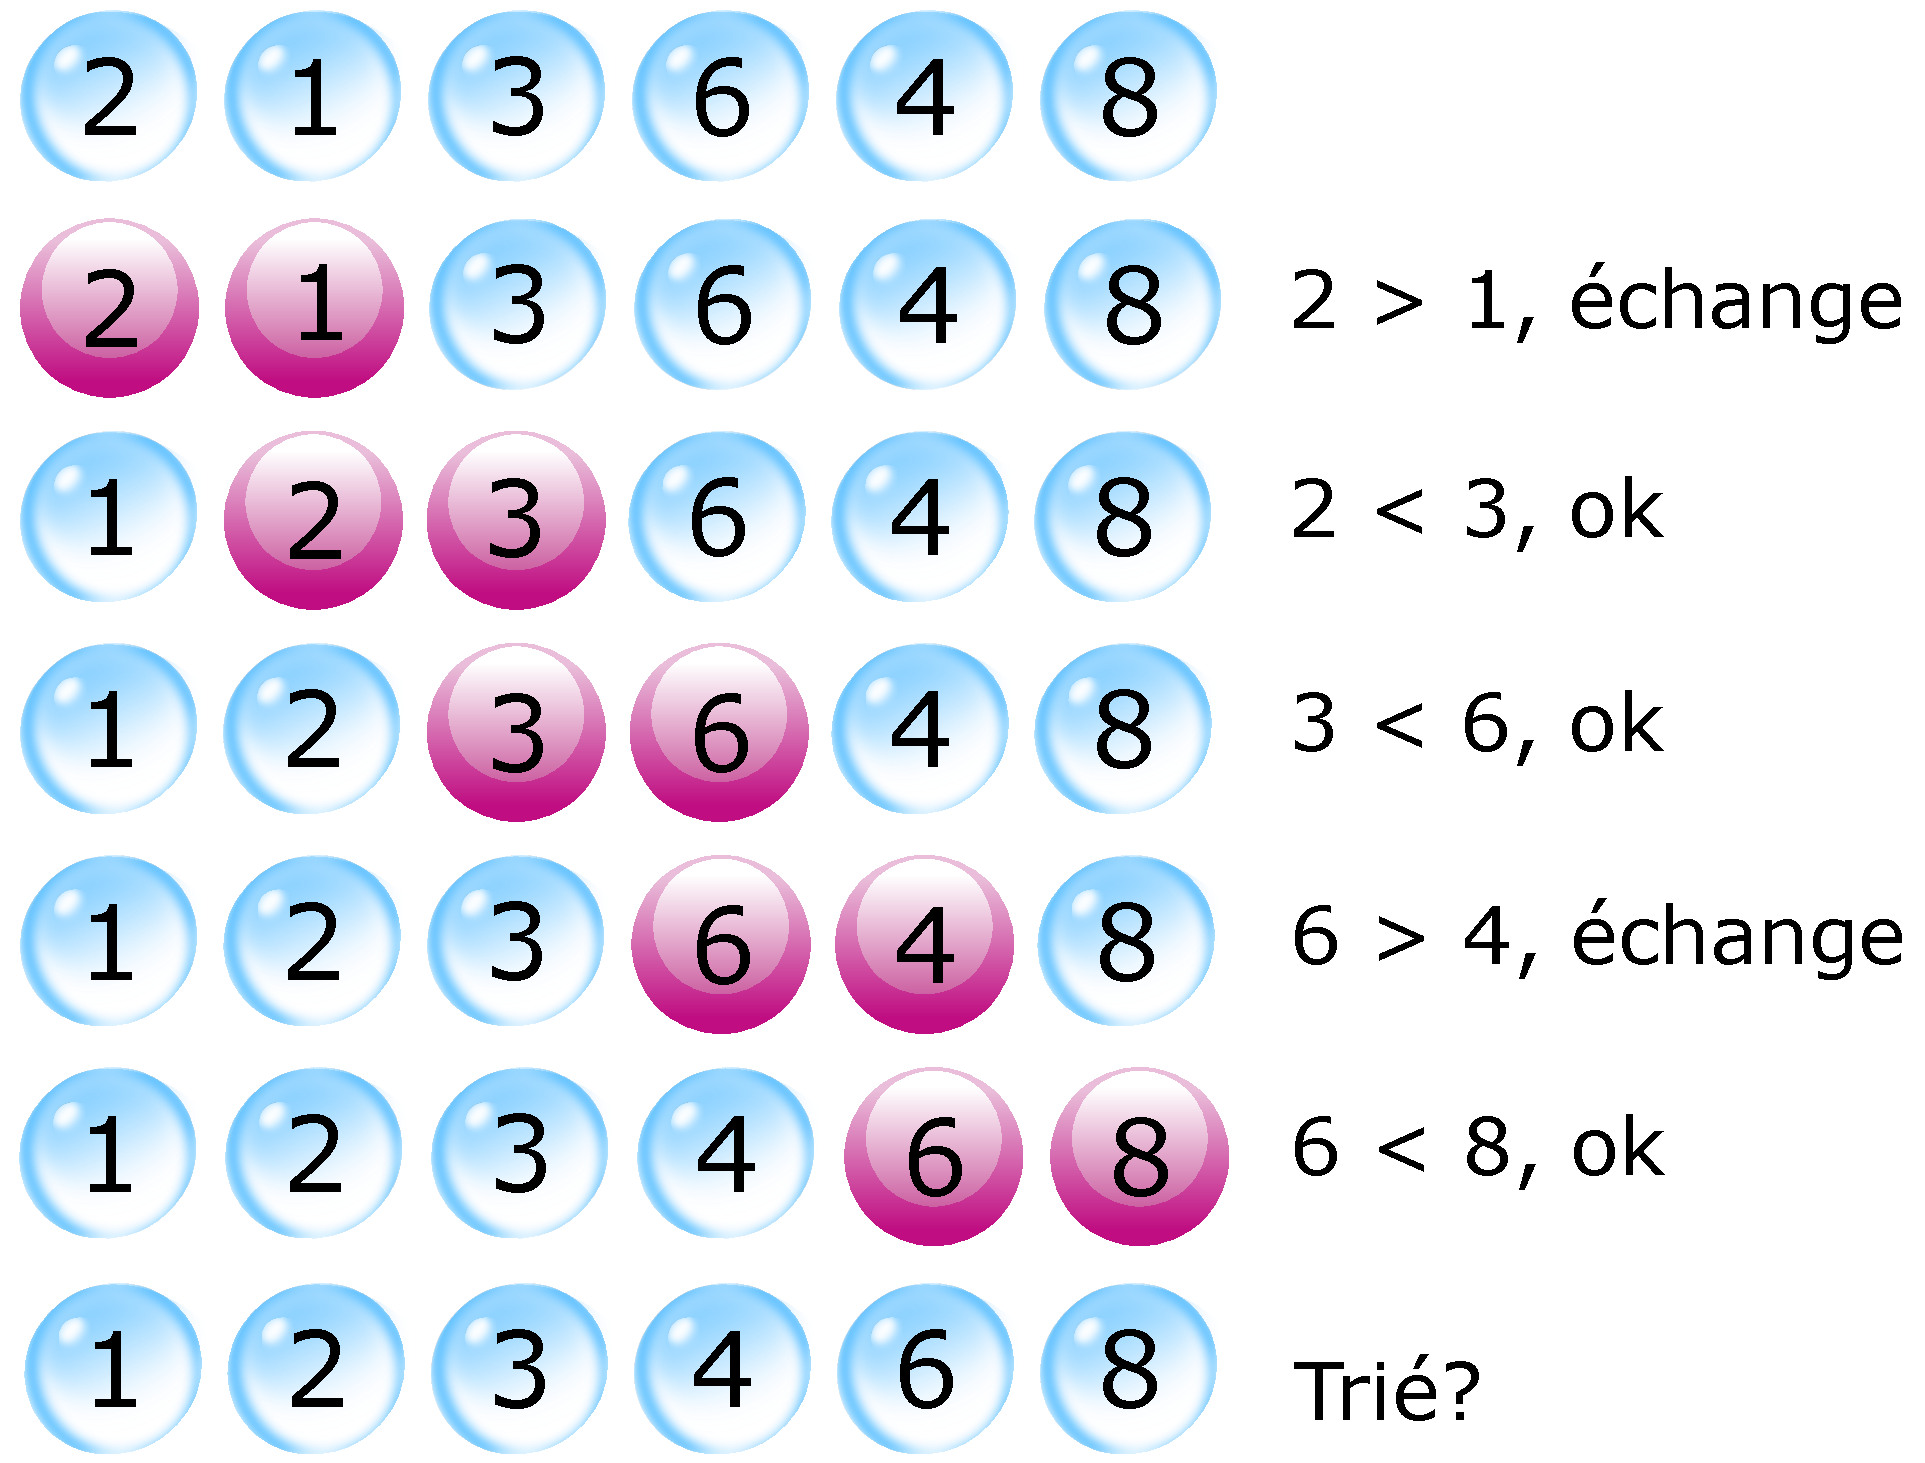
\includegraphics[scale=0.22]{figs/bubble_sort2_13}
\end{figure}
}

\end{frame}



\begin{frame}{Le tri par sélection}


\begin{figure}
\includegraphics[scale=0.18]{figs/dinosaur.png}
\end{figure}

\end{frame}

\begin{frame}{Le tri par sélection}{Principe}

\begin{itemize}
\item[1]On définit une fenêtre qui couvre l'ensemble du tableau.
\item[2]A chaque étape, on réduit d'une case la fenêtre en allant vers la fin.
\item[4]On échange la première case de la fenêtre avec la valeur minimum de la fenêtre.
\item[3]Quand la fenêtre correspond à l'élément de fin, c'est trié.
\end{itemize}
%On va successivement réduire la taille d'une fenêtre allant du début à la fin du tableau (jusqu'à ne couvrir que la dernière case).

\end{frame}

\begin{frame}{Le tri par sélection}{En images}

%A chaque étape, on échange le contenu de la première case de la fenêtre avec la valeur minimum de celle-ci.

\only<1>{
\begin{figure}
\centering
\includegraphics[scale=0.30]{figs/selection_sort_1}
\end{figure}
}

\only<2>{
\begin{figure}
\centering
\includegraphics[scale=0.30]{figs/selection_sort_2}
\end{figure}
}
\only<3>{
\begin{figure}
\centering
\includegraphics[scale=0.30]{figs/selection_sort_3}
\end{figure}
}

\only<4>{
\begin{figure}
\centering
\includegraphics[scale=0.30]{figs/selection_sort_4}
\end{figure}
}

\only<5>{
\begin{figure}
\centering
\includegraphics[scale=0.30]{figs/selection_sort_5}
\end{figure}
}

\only<6>{
\begin{figure}
\centering
\includegraphics[scale=0.30]{figs/selection_sort_6}
\end{figure}
}
\only<7>{
\begin{figure}
\centering
\includegraphics[scale=0.30]{figs/selection_sort_7}
\end{figure}
}






\end{frame}
\begin{frame}{Le tri par insertion}

\begin{figure}
\centering
\includegraphics[scale=0.3]{figs/insertion_cards}
\end{figure}
\end{frame}

\begin{frame}{Le tri par insertion}{Principe}
\textit{C'est la manière dont on trie naturellement les cartes que l'on a en main!
}
\begin{itemize}
\item[1]On définit une fenêtre qui ne contient que le premier élément
\item[2]On parcourt le tableau
\item[3]A chaque étape du parcours, on agrandit la fenêtre d'une case vers la fin
\item[4]On place l'élément courant à sa place dans la fenêtre de manière à ce qu'elle soit triée.
\end{itemize}

\end{frame}

\begin{frame}{Le tri par insertion}{En images}

\only<1>{
\begin{figure}
\centering
\includegraphics[scale=0.30]{figs/insertion_sort_1}
\end{figure}
}

\only<2>{
\begin{figure}
\centering
\includegraphics[scale=0.30]{figs/insertion_sort_2}
\end{figure}
}
\only<3>{
\begin{figure}
\centering
\includegraphics[scale=0.30]{figs/insertion_sort_3}
\end{figure}
}

\only<4>{
\begin{figure}
\centering
\includegraphics[scale=0.30]{figs/insertion_sort_4}
\end{figure}
}

\only<5>{
\begin{figure}
\centering
\includegraphics[scale=0.30]{figs/insertion_sort_5}
\end{figure}
}

\only<6>{
\begin{figure}
\centering
\includegraphics[scale=0.30]{figs/insertion_sort_6}
\end{figure}
}


\end{frame}




\begin{frame}{A vous de jouer!}

\end{frame}

\begin{frame}{Bilan}
Dans ce cours, nous avons vu
\begin{itemize}
\item pourquoi trier,
\item plusieurs algorithmes de tri (lents),
\item des éléments pour étudier leur efficacité.
\end{itemize}
\end{frame}

\begin{frame}[fragile]{Bonus}{Le Bogosort(ou tri stupide)}
Un algorithme de tri diablement inefficace:\newline
$\Rightarrow$ Tant que mon tableau n'est pas trié, je le mélange aléatoirement!

\pause
\begin{lstlisting}

void bogosort(int [] tab){
  while(!sorted(tab)){
    shuffle(tab)
  }
}
\end{lstlisting}
\pause
Implémentez les méthodes \texttt{shuffle} et \texttt{sorted!}


\end{frame}

\begin{frame}[fragile]{Bogosort}{Solution}

\begin{lstlisting}
 boolean sorted(int [] tab){
     for(int i = 0; i < tab.length;i++){
        if(tab[i] > tab [i+1]){
        return false;
        }
     }
     return true;
 }
 

 \end{lstlisting}

\pause

\begin{lstlisting}
void shuffle(int [] tab){
  int idx, idx2;
  for (int i = 0; i < tab.length; i++) {
   idx = ((int) (Math.random() * i.length);
   idx2 = (int) (Math.random() * i.length);
   swap(idx,idx2);
}

 \end{lstlisting}


\end{frame}

\end{document}